\documentclass[tikz,border=6pt]{standalone}

\usepackage[T1]{fontenc}
\usepackage{lmodern}
\usepackage{amsmath}
\usepackage{xcolor}
\usetikzlibrary{shapes,arrows,positioning,calc}

\begin{document}
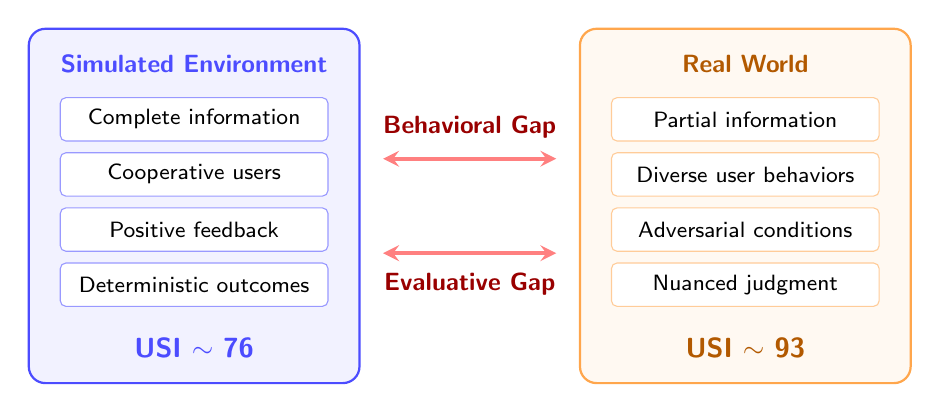
\begin{tikzpicture}[
    simbox/.style={rectangle, draw=#1!70, fill=#1!5, minimum width=4.2cm, minimum height=4.5cm, align=center, rounded corners=6pt, thick},
    prop/.style={rectangle, draw=#1!40, fill=white, minimum width=3.4cm, minimum height=0.55cm, align=center, font=\footnotesize\sffamily, rounded corners=2pt, thin},
    gaplbl/.style={font=\small\sffamily\bfseries, text=red!60!black},
    gaparr/.style={<->, >=stealth, thick, color=red!50, line width=1.5pt}
]
% Simulated Environment
\node[simbox=blue] (sim) at (-3.5,0) {};
\node[font=\small\sffamily\bfseries, text=blue!70] at (-3.5,1.8) {Simulated Environment};
\node[prop=blue] at (-3.5,1.1) {Complete information};
\node[prop=blue] at (-3.5,0.4) {Cooperative users};
\node[prop=blue] at (-3.5,-0.3) {Positive feedback};
\node[prop=blue] at (-3.5,-1.0) {Deterministic outcomes};
\node[font=\sffamily\bfseries, text=blue!70] at (-3.5,-1.8) {USI $\sim$ 76};

% Real World
\node[simbox=orange] (real) at (3.5,0) {};
\node[font=\small\sffamily\bfseries, text=orange!70!black] at (3.5,1.8) {Real World};
\node[prop=orange] at (3.5,1.1) {Partial information};
\node[prop=orange] at (3.5,0.4) {Diverse user behaviors};
\node[prop=orange] at (3.5,-0.3) {Adversarial conditions};
\node[prop=orange] at (3.5,-1.0) {Nuanced judgment};
\node[font=\sffamily\bfseries, text=orange!70!black] at (3.5,-1.8) {USI $\sim$ 93};

% Gap labels
\draw[gaparr] (-1.1,0.6) -- (1.1,0.6);
\node[gaplbl] at (0,1.0) {Behavioral Gap};
\draw[gaparr] (-1.1,-0.6) -- (1.1,-0.6);
\node[gaplbl] at (0,-1.0) {Evaluative Gap};
\end{tikzpicture}
\end{document}